\documentclass[11pt]{article}
\usepackage{fullpage,amsthm,amsfonts,amssymb,epsfig,amsmath,times,amsthm,array,graphicx}
\newcolumntype{C}{>$c<$}
\usepackage[shortlabels]{enumitem}
\usepackage{mathtools}
\graphicspath{ {images/} }
\DeclarePairedDelimiter\ceil{\lceil}{\rceil}
\DeclarePairedDelimiter\floor{\lfloor}{\rfloor}

\newtheorem{theorem}{Theorem}
\newtheorem{claim}[theorem]{Claim}
\newtheorem*{claim*}{Claim}

\begin{document}

\begin{center}
{\bf\Large CMPS 130 -- Spring Quarter 2017 --  Homework 1}\\
Christopher Hsiao -- chhsiao@ucsc.edu -- 1398305\\
\end{center}



\section{Exercises from pages 25, 26, and 27 of the book: 0.1 through 0.9}
\subsection*{0.1} 
Examine the following formal descriptions of sets so that you understand which members they contain. Write a short informal English description of each set.

\begin{enumerate}[a.]
\item The infinite set of all positive odd integers, or the set of all odd natural numbers.
\item The infinite set of all even integers.
\item The infinite set of all even natural numbers.
\item The infinite set of all even natural numbers, and all natural numbers which are multiples of 3.
\item The infinite set containing all palindromic bit strings.
\item The finite set containing any integer $n$ and $n+1$. ========
\end{enumerate}

\subsection*{0.2}
Write formal descriptions of the following sets.

\begin{enumerate}[a.]
\item $\{1, 10, 100\}$
\item $\{n | n > 5 \text{ for some } n \in \mathbb{Z}\}$
\item $\{1, 2, 3, 4\}$
\item $\{aba\}$
\item $\{""\}$
\item $\{ \}$
\end{enumerate}

\subsection*{0.3}
Let $A$ be the set $\{x, y, z\}$ and $B$ be the set $\{x, y\}$.

\begin{enumerate}[a.]
\item No.
\item Yes.
\item $\{x, y, z\}$
\item $\{x, y\}$
\item \{\{x,x\}, \{x,y\}, \{y,x\}, \{y, y\}, \{z, x\}, \{z, y\}\}
\item \{\{\}, \{x\}, \{y\}, \{x,y\}\}
\end{enumerate}

\subsection*{0.4}
If $A$ has $a$ elements, and $B$ has $b$ elements, how many elements are in $A \times B$? Explain your answer.\\
\begin{claim*}
$|A \times B| = a \cdot b$ 
\end{claim*}
\begin{proof}
This is because we assign every element of the set $A$ to every element in the set $B$. That means, each element in the set $A$, such as $A_i$, has $b$ pairings made. Thus, if there are $b$ pairings made with every element in $A$, then there are $a$ pairings, each of size $b$, which yields $a \cdot b$ number of pairings made. 
\end{proof}

\subsection*{0.5}
If $C$ is a set with $c$ elements, how many elements are in the power set of $C$? Explain your answer.\\
\\
First, we will define the power set of $C$ as $P_C$. 
\begin{claim*}
$|P_C| = 2^{c}$
\end{claim*}
\begin{proof}

\end{proof}

\subsection*{0.6}
Let X be the set $\{1, 2, 3, 4, 5\}$ and $Y$ be the set $\{6, 7, 8, 9, 10\}$. The unary function $f: X \rightarrow Y$ and the binary function $g: X \times Y \rightarrow Y$ are described.

\begin{enumerate}[a.]
\item 7
\item $D: [6,7]$, $R: [1,5]$
\item 6
\item $D: [6,10]$, $R: [1,5]$
\item 8
\end{enumerate}

\subsection*{0.7}
For each part, give a relation that satisfies the condition. Let A = \{x, y, z\}.
\begin{enumerate}[a.]
\item Reflexive, Symmetric, but not Transitive. \\
Let $R$ = \{(x, x), (y, y), (z, z), (x, y), (y, x), (y, z), (z, y)\}\\
$R$ is reflexive, since (x, x), (y, y), (z, z) $\in R$.\\
$R$ is symmetric, since (x, y), (y, x), (y, z), (z, y) $\in R$.\\
$R$ is not transitive, since (x, y) (y, z) $\in R$, but (x, z) $\notin R$.
\item Reflexive, Transitive, but not Symmetric. \\
Let $R$ = \{(x, x), (y, y), (z, z), (x, y), (y, z), (x, z)\}\\
$R$ is reflexive, since (x, x), (y, y), (z, z) $\in R$.\\
$R$ is transitive, since (x, y), (y, z), (x, z) $\in R$, where (x, y) and (y, z) $\implies$ (x, z)\\
$R$ is not symmetric, since (x, y), (y, z), (x, z) $\in R$, but (y, x), (z, y), (z, x) $\notin R$.
\item Symmetric, Transitive, but not Reflexive.\\
Let $R$ = \{(x, y), (y, x), (y, z), (z, y), (x, z), (z, x)\}\\
$R$ is symmetric, since (x, y), (y, x), (y, z), (x, z), (z, x) $\in R$.\\
$R$ is transitive, since (x, y), (y, z), (z, x) $\in R$, where (x, y) and (y, z) $\implies$ (z, x).\\
$R$ is not reflexive, since (x, x), (y, y), (z, z) $\notin R$.
\end{enumerate}

\subsection*{0.8}
Consider the undirected graph $G=(V,E) where V$ , the set of nodes, is \{1, 2, 3, 4\} and $E$, the set of edges, is \{\{1, 2\}, \{2, 3\}, \{1, 3\}, \{2, 4\}, \{1, 4\}\}. Draw the graph $G$. What are the degrees of each node? Indicate a path from node 3 to
node 4 on your drawing of $G$.\\
\begin{center} 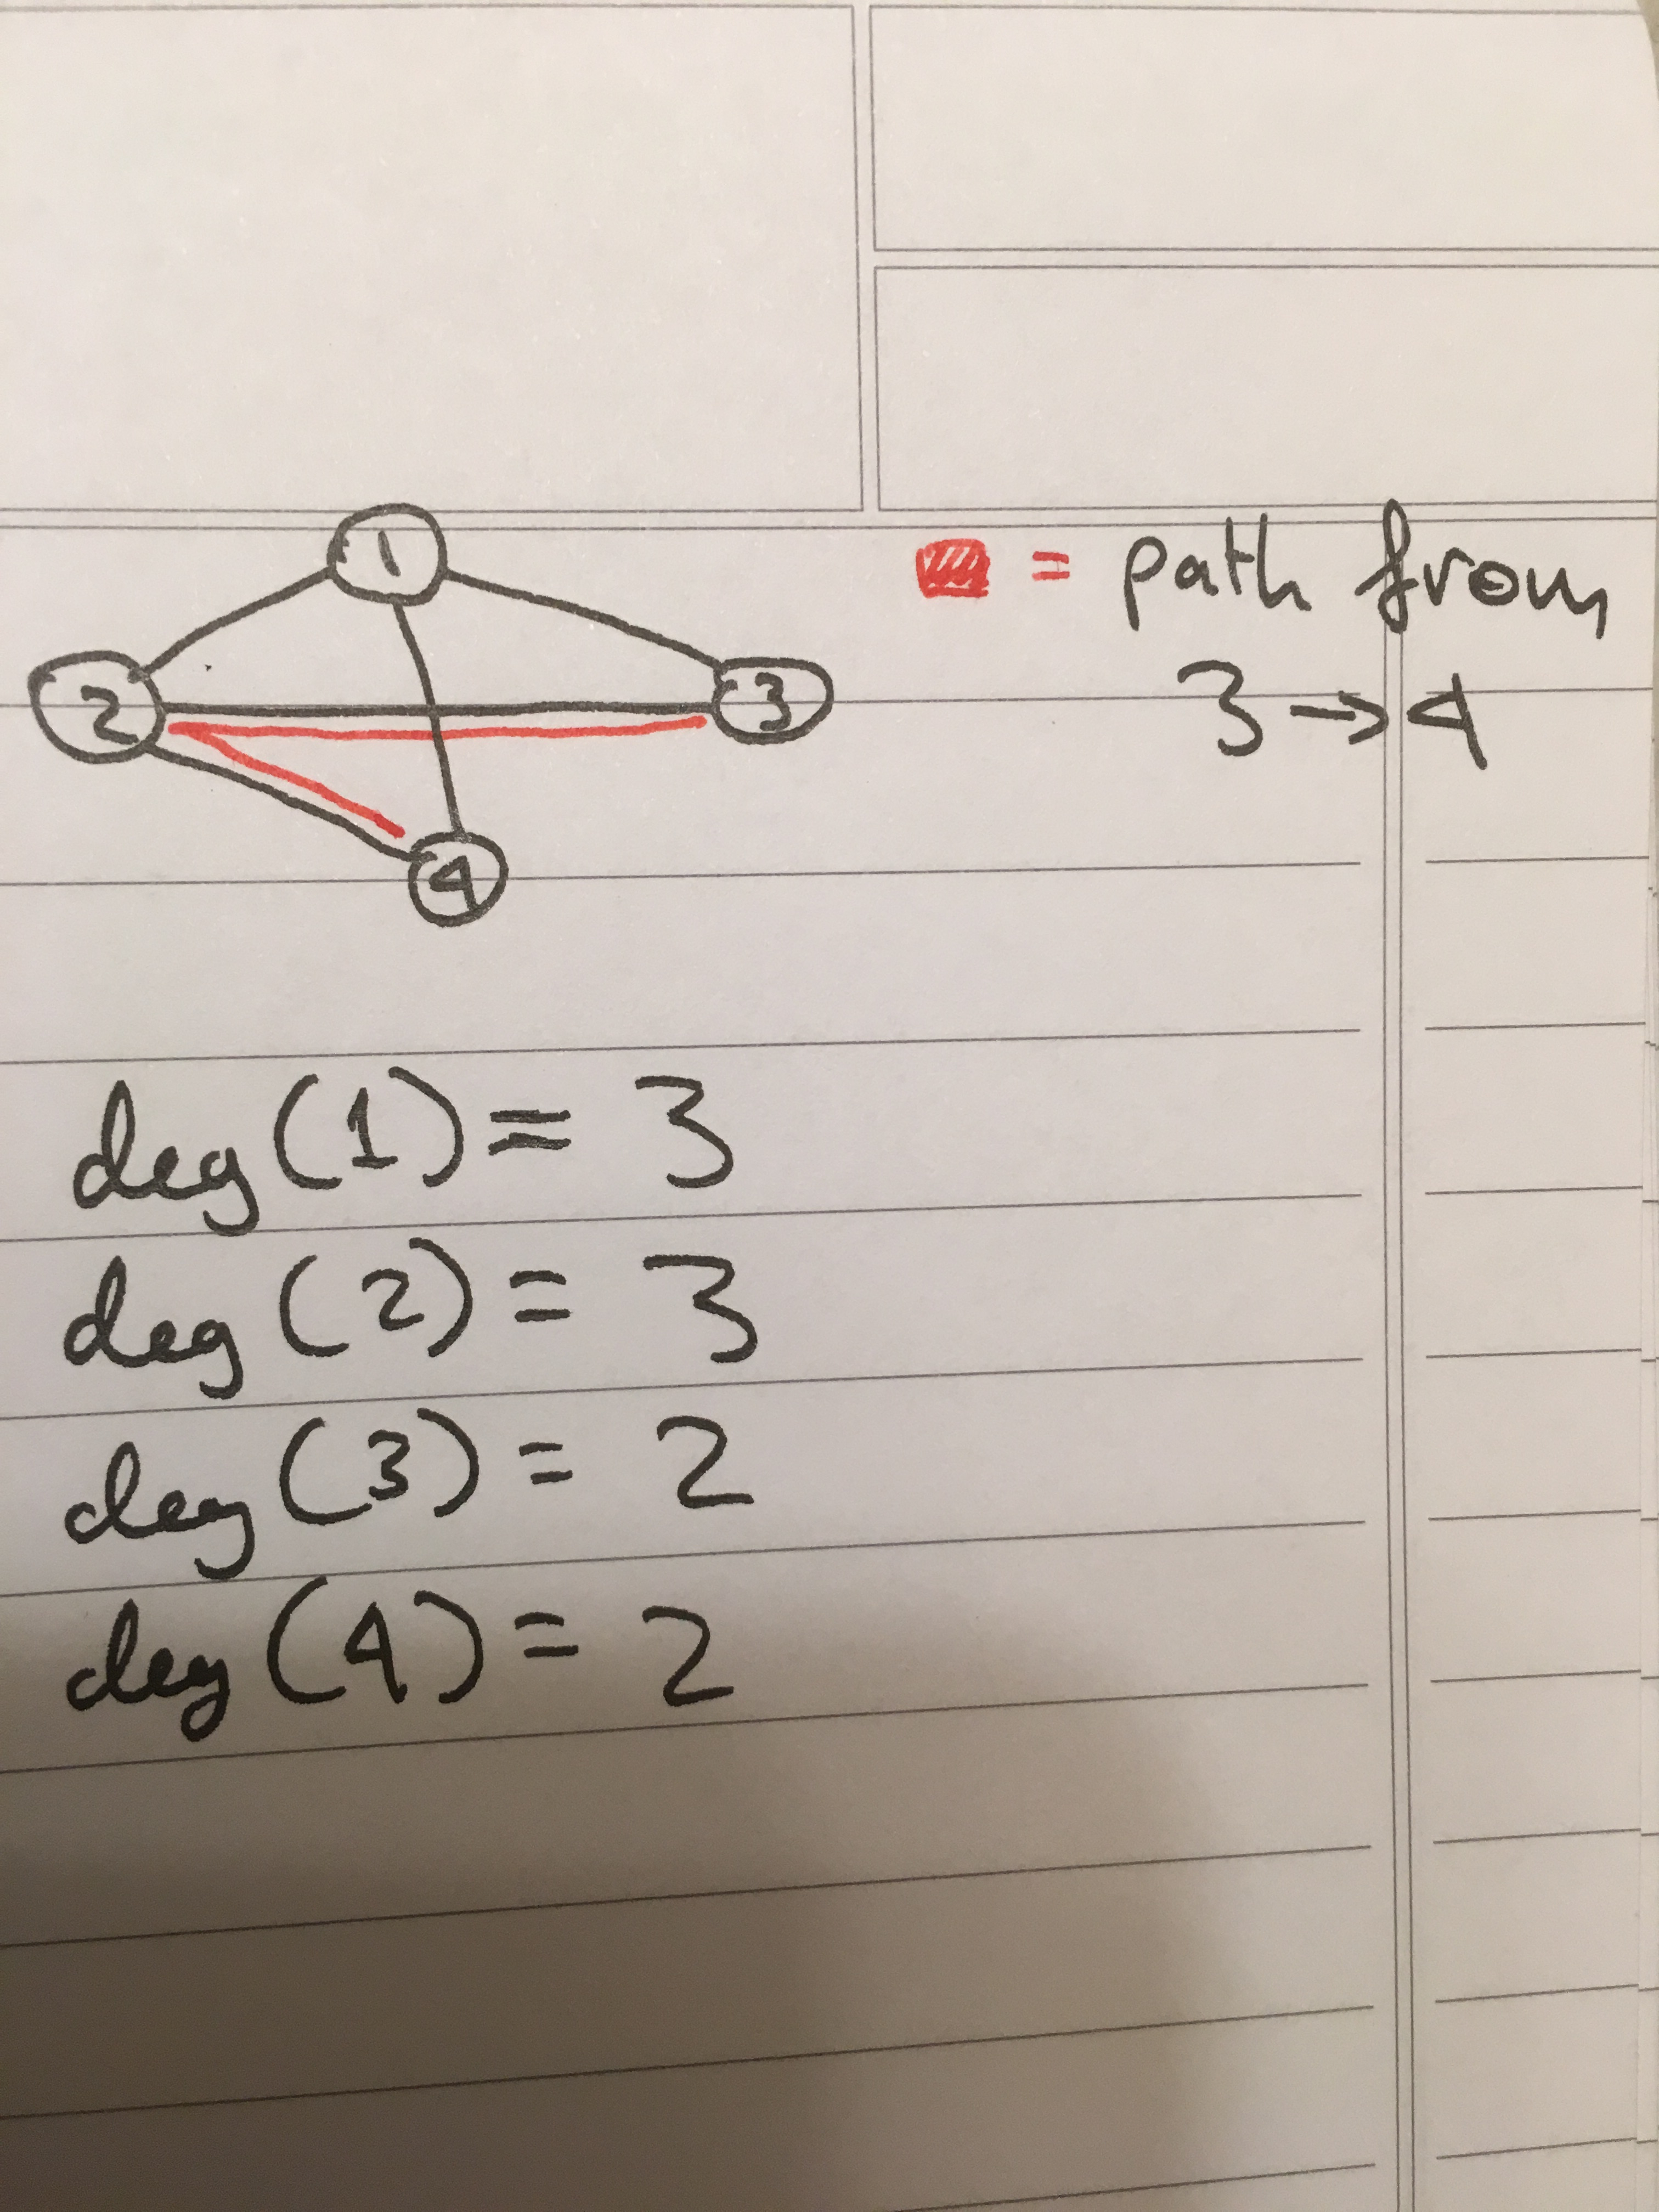
\includegraphics[width=10cm,height=10cm,keepaspectratio]{exer08} \end{center}

\pagebreak
\subsection*{0.9}
Write a formal description of the following graph.
\begin{center} 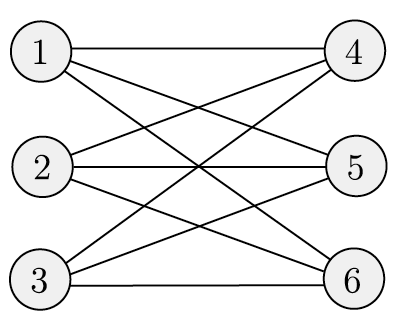
\includegraphics[width=6cm,height=6cm,keepaspectratio]{exer09} \end{center}
\{\{1, 2, 3, 4, 5, 6\}, \{(1, 4), (1, 5), (1, 6), (2, 4), (2, 5), (2, 6), (3, 4), (3, 5), (3, 6)\}\}

\section{Problems page 27 in 2nd ed 0.10 through 0.12}

\end{document}
